% Options for packages loaded elsewhere
\PassOptionsToPackage{unicode}{hyperref}
\PassOptionsToPackage{hyphens}{url}
\PassOptionsToPackage{dvipsnames,svgnames,x11names}{xcolor}
%
\documentclass[
]{agujournal2019}

\usepackage{amsmath,amssymb}
\usepackage{iftex}
\ifPDFTeX
  \usepackage[T1]{fontenc}
  \usepackage[utf8]{inputenc}
  \usepackage{textcomp} % provide euro and other symbols
\else % if luatex or xetex
  \usepackage{unicode-math}
  \defaultfontfeatures{Scale=MatchLowercase}
  \defaultfontfeatures[\rmfamily]{Ligatures=TeX,Scale=1}
\fi
\usepackage{lmodern}
\ifPDFTeX\else  
    % xetex/luatex font selection
\fi
% Use upquote if available, for straight quotes in verbatim environments
\IfFileExists{upquote.sty}{\usepackage{upquote}}{}
\IfFileExists{microtype.sty}{% use microtype if available
  \usepackage[]{microtype}
  \UseMicrotypeSet[protrusion]{basicmath} % disable protrusion for tt fonts
}{}
\makeatletter
\@ifundefined{KOMAClassName}{% if non-KOMA class
  \IfFileExists{parskip.sty}{%
    \usepackage{parskip}
  }{% else
    \setlength{\parindent}{0pt}
    \setlength{\parskip}{6pt plus 2pt minus 1pt}}
}{% if KOMA class
  \KOMAoptions{parskip=half}}
\makeatother
\usepackage{xcolor}
\setlength{\emergencystretch}{3em} % prevent overfull lines
\setcounter{secnumdepth}{5}
% Make \paragraph and \subparagraph free-standing
\ifx\paragraph\undefined\else
  \let\oldparagraph\paragraph
  \renewcommand{\paragraph}[1]{\oldparagraph{#1}\mbox{}}
\fi
\ifx\subparagraph\undefined\else
  \let\oldsubparagraph\subparagraph
  \renewcommand{\subparagraph}[1]{\oldsubparagraph{#1}\mbox{}}
\fi


\providecommand{\tightlist}{%
  \setlength{\itemsep}{0pt}\setlength{\parskip}{0pt}}\usepackage{longtable,booktabs,array}
\usepackage{calc} % for calculating minipage widths
% Correct order of tables after \paragraph or \subparagraph
\usepackage{etoolbox}
\makeatletter
\patchcmd\longtable{\par}{\if@noskipsec\mbox{}\fi\par}{}{}
\makeatother
% Allow footnotes in longtable head/foot
\IfFileExists{footnotehyper.sty}{\usepackage{footnotehyper}}{\usepackage{footnote}}
\makesavenoteenv{longtable}
\usepackage{graphicx}
\makeatletter
\def\maxwidth{\ifdim\Gin@nat@width>\linewidth\linewidth\else\Gin@nat@width\fi}
\def\maxheight{\ifdim\Gin@nat@height>\textheight\textheight\else\Gin@nat@height\fi}
\makeatother
% Scale images if necessary, so that they will not overflow the page
% margins by default, and it is still possible to overwrite the defaults
% using explicit options in \includegraphics[width, height, ...]{}
\setkeys{Gin}{width=\maxwidth,height=\maxheight,keepaspectratio}
% Set default figure placement to htbp
\makeatletter
\def\fps@figure{htbp}
\makeatother
% definitions for citeproc citations
\NewDocumentCommand\citeproctext{}{}
\NewDocumentCommand\citeproc{mm}{%
  \begingroup\def\citeproctext{#2}\cite{#1}\endgroup}
\makeatletter
 % allow citations to break across lines
 \let\@cite@ofmt\@firstofone
 % avoid brackets around text for \cite:
 \def\@biblabel#1{}
 \def\@cite#1#2{{#1\if@tempswa , #2\fi}}
\makeatother
\newlength{\cslhangindent}
\setlength{\cslhangindent}{1.5em}
\newlength{\csllabelwidth}
\setlength{\csllabelwidth}{3em}
\newenvironment{CSLReferences}[2] % #1 hanging-indent, #2 entry-spacing
 {\begin{list}{}{%
  \setlength{\itemindent}{0pt}
  \setlength{\leftmargin}{0pt}
  \setlength{\parsep}{0pt}
  % turn on hanging indent if param 1 is 1
  \ifodd #1
   \setlength{\leftmargin}{\cslhangindent}
   \setlength{\itemindent}{-1\cslhangindent}
  \fi
  % set entry spacing
  \setlength{\itemsep}{#2\baselineskip}}}
 {\end{list}}
\usepackage{calc}
\newcommand{\CSLBlock}[1]{\hfill\break\parbox[t]{\linewidth}{\strut\ignorespaces#1\strut}}
\newcommand{\CSLLeftMargin}[1]{\parbox[t]{\csllabelwidth}{\strut#1\strut}}
\newcommand{\CSLRightInline}[1]{\parbox[t]{\linewidth - \csllabelwidth}{\strut#1\strut}}
\newcommand{\CSLIndent}[1]{\hspace{\cslhangindent}#1}

\usepackage{url} %this package should fix any errors with URLs in refs.
\usepackage{lineno}
\usepackage[inline]{trackchanges} %for better track changes. finalnew option will compile document with changes incorporated.
\usepackage{soul}
\linenumbers
\makeatletter
\@ifpackageloaded{float}{}{\usepackage{float}}
\floatstyle{plain}
\@ifundefined{c@chapter}{\newfloat{suppfig}{h}{losuppfig}}{\newfloat{suppfig}{h}{losuppfig}[chapter]}
\floatname{suppfig}{Figure S}
\newcommand*\quartosuppfigref[1]{Figure \hyperref[#1]{S\ref{#1}}}
\@ifpackageloaded{caption}{}{\usepackage{caption}}
\DeclareCaptionLabelFormat{quartosuppfigreflabelformat}{#1#2}
\captionsetup[suppfig]{labelformat=quartosuppfigreflabelformat}
\newcommand*\listofsuppfigs{\listof{suppfig}{List of Supplementary Figures}}
\makeatother
\makeatletter
\@ifpackageloaded{caption}{}{\usepackage{caption}}
\AtBeginDocument{%
\ifdefined\contentsname
  \renewcommand*\contentsname{Table of contents}
\else
  \newcommand\contentsname{Table of contents}
\fi
\ifdefined\listfigurename
  \renewcommand*\listfigurename{List of Figures}
\else
  \newcommand\listfigurename{List of Figures}
\fi
\ifdefined\listtablename
  \renewcommand*\listtablename{List of Tables}
\else
  \newcommand\listtablename{List of Tables}
\fi
\ifdefined\figurename
  \renewcommand*\figurename{Figure}
\else
  \newcommand\figurename{Figure}
\fi
\ifdefined\tablename
  \renewcommand*\tablename{Table}
\else
  \newcommand\tablename{Table}
\fi
}
\@ifpackageloaded{float}{}{\usepackage{float}}
\floatstyle{ruled}
\@ifundefined{c@chapter}{\newfloat{codelisting}{h}{lop}}{\newfloat{codelisting}{h}{lop}[chapter]}
\floatname{codelisting}{Listing}
\newcommand*\listoflistings{\listof{codelisting}{List of Listings}}
\makeatother
\makeatletter
\makeatother
\makeatletter
\@ifpackageloaded{caption}{}{\usepackage{caption}}
\@ifpackageloaded{subcaption}{}{\usepackage{subcaption}}
\makeatother
\ifLuaTeX
  \usepackage{selnolig}  % disable illegal ligatures
\fi
\usepackage{bookmark}

\IfFileExists{xurl.sty}{\usepackage{xurl}}{} % add URL line breaks if available
\urlstyle{same} % disable monospaced font for URLs
\hypersetup{
  pdftitle={Effects of Riparian Grazing on Distinct Phosphorus Sources},
  pdfauthor={Alexander J Koiter; Tamaragh Y Malone},
  pdfkeywords={Phosphorus, Grazing, Riparian},
  colorlinks=true,
  linkcolor={blue},
  filecolor={Maroon},
  citecolor={Blue},
  urlcolor={Blue},
  pdfcreator={LaTeX via pandoc}}

\journalname{TBD}

\draftfalse

\begin{document}
\title{Effects of Riparian Grazing on Distinct Phosphorus Sources}

\authors{Alexander J Koiter\affil{1}, Tamaragh Y Malone\affil{2}}
\affiliation{1}{Brandon University, Department of Geography and
Environment, Brandon, MB, }\affiliation{2}{Brandon University,
Department of Biology, Brandon, MB, }
\correspondingauthor{Alexander J Koiter}{koitera@brandonu.ca}


\begin{abstract}
Riparian areas play an important role in maintaining water quality in
agricultural watersheds by buffering sediment, nutrients, and other
pollutants. Additionally, these areas are also an important sources of
forage, particularly during drought. Recent studies have shown that
riparian areas are less effective buffers and, in some cases, are a net
source of phosphorus (P) in cold climates. The repeated freeze-thaw
cycles increase the availability of P in both the vegetation and soil
sources. Cattle grazing or harvesting of riparian areas prior to the
onset of winter conditions may be a viable management practice to reduce
the loss of P during the spring snowmelt. This study measured the
water-extractable phosphorus (WEP) in four distinctive sources: biomass,
litter, organic layer, and Ah horizon. Overall, the Ah (0-10cm) soil was
the largest (\textasciitilde44\%) source of WEP; however, the biomass
(i.e., standing vegetation) was a considerable proportion
(\textasciitilde25\%) of the total. In addition to control plots, the
riparian areas were subjected to grazing, high density grazing, and
mowing treatments. Findings revealed significant reductions in biomass
WEP with high density grazing and mowing treatments, particularly in
lower riparian zones. There were no detectable changes in the other
sources of WEP. This suggests that autumn short-term grazing may be a
mechanism to use this important forage resource and reduce the potential
P loss during the snowmelt period.
\end{abstract}

\section*{Plain Language Summary}
Riparian areas are important for keeping water clean in agricultural
watersheds because they help filter out sediment, nutrients, and other
pollutants. Some recent studies found that in cold climates, like the
Canadian Prairies, riparian areas are not as effective at filtering out
nutrients. Because of the freez and thaw of soil and vegetation during
the spring snowmelt riparian areas can be a source of phosphorus to the
water instead of removing it. To see if we can reduce the loss of
phosphorus we looked at different sources of phosphorus in riparian
areas including plants, dead vegetation, and soil. Cattle grazing and
mowing were tested as ways of managing the riparian areas. Both cattle
grazing and mowing reduced the amount of plant-based phosphorus without
increasing the other sources. This shows that letting cows graze in the
fall might be a good way to use this forage and also prevent too much
phosphorus from getting into the water when the snow melts in the
spring.



\textbf{Core ideas}

\begin{itemize}
\tightlist
\item
  Biomass and litter are substantial sources of WEP in riparian areas
\item
  Autumn cattle grazing and mowing treatments reduced the amount of WEP
  in riparian biomass
\item
  No Measurable change in the amount of WEP in the litter, organic
  layer, or Ah horizon post grazing
\item
  Large spatial variability in WEP exists in riparian areas
\end{itemize}

\textbf{Abbreviations}

FTC, freeze-thaw cycle; MBFI, Manitoba Beef and Forage Initiatives; P,
phosphorus; WEP, water extractable phosphorus

\section{Introduction}\label{introduction}

Riparian areas are transitional areas within watersheds that are
important for the health and functionality of both terrestrial and
aquatic environments (Gregory et al., 1991). Riparian areas buffer the
delivery of water, sediment, nutrients, and pollutants from upland areas
before they enter surface water and are commonly conserved, restored, or
managed in an effort to improve downstream water quality (Dillaha et
al., 1989; Borin et al., 2005; Dorioz et al., 2006). Additionally,
riparian areas also provide essential habitat and corridors for range of
plants and animals, particularly in highly fragmented or modified
landscapes (Montgomery, 1996; Luther et al., 2008; Forio et al., 2020).
Within the aquatic environment riparian vegetation stabilizes banks,
regulates water temperature, provides woody debris and other organic
matter, and generally supports aquatic habitat and biodiversity
(Studinski et al., 2012; Dauwalter et al., 2018; Verdonschot and
Verdonschot, 2024). Beyond ecosystem services, riparian zones can offer
recreational opportunities (e.g., hiking, fishing, canoeing, foraging)
and are key components of the agricultural landscape. Beyond improving
water quality, riparian areas benefit agricultural production through
providing habitat for beneficial organisms (e.g., pollination, pest
control), a source of forage during drought (livestock health and
productivity), and other opportunities (e.g., agroforestry, carbon
sequestration) (Cole et al., 2015, 2020).

Increasing frequency and extent of algal blooms are typically linked to
increased nutrient loading into lake and rivers. Of particular concern
is phosphorus (P) loading as this is generally the limiting nutrient in
fresh water systems (Schindler et al., 2012). There have been many lab
and field studies demonstrating the role and functionality of riparian
areas to reduce P loading to surface water in agricultural settings (Yu
et al., 2019). Infiltration, absorption, biological uptake, microbial
activity, and sedimentation are the key processes that intercept and
buffer the delivery of P (Lacas et al., 2005; Owens et al., 2007;
McGuire and McDonnell, 2010). Convergence within the landscape coupled
with climatic/weather conditions creates variability in hydrologic
conditions and pathways reducing the buffering capacity of riparian
areas and ultimately resulting in reduced, inconsistent and/or
unsustainable reductions in P loading relative to many controlled
experimental studies (Roberts et al., 2012; Habibiandehkordi et al.,
2017).

In cold climates, the the reduced infiltration due frozen ground,
limited vegetation uptake, and low microbial activity coupled with a
flashy hydrograph during snowmelt creates conditions that further
compromise buffering capacity of riparian areas (Kieta et al., 2018;
Nsenga Kumwimba et al., 2023). Additionally, research increasingly shows
that riparian areas can contribute P (i.e., net source) to the
surrounding environment (Roberts et al., 2012). The sources of this
riparian-derived P are soil and vegetation. As soil P content increases
over time, so does the risk of P loss through leaching and runoff
(Habibiandehkordi et al., 2019). This process can be intensified during
periods of inundation, in addition to a longer period of soil-water
contact, the solubility of iron-bound P increases as redox conditions
lower (Carlyle and Hill, 2001; Young and Briggs, 2008). Furthermore,
mineralization of P from dead vegetation near the soil surface will also
contribute to the P available to be lost during runoff (Liu et al.,
2019b). Both the soil and vegetation P sources can also be affected by
freeze-thaw cycles (FTC). Repeated FTCs result in the cell disruption of
microbial and plant biomass, releasing inter-cellular P to the
surrounding environment (Kieta and Owens, 2019). Removing or harvesting
the vegetation prior to freeze-up will help draw-down the soil P content
and reduce the amount of vegetation contributing P during the spring
snowmelt.

Environmental conditions, particularly hydrological and temperature
fluctuations, create considerable spatial and temporal variability in
both P sources, transformations, and transport processes. These hot
spots and hot moments in riparian processes create challenges for
effective management (McClain et al., 2003; Vidon et al., 2010). From a
surface water quality perspective, understanding the near-surface P
distribution, both vertically and longitudinal will help in the
development and identification of best management practices for reducing
P loading. There are often four identifiable sources of near-surface P:
1) biomass consisting of living standing vegetation; 2) litter
consisting of fresh (\textasciitilde1-3 yrs) residues; 3) partially to
well decomposed organic material; and 4) mineral soil (Reid et al.,
2018). A better understanding of the spatial variability and relative
contributions of the different sources of P is needed assess the risks
and benefits of different management strategies.

Management of riparian areas to maintain or enhance the buffering
capacity of P is typically needed in the long term. Unlike nitrogen (N)
where there can be significant loss of N to the atmosphere through the
processes of nitrification and denitrification to offset the continued
input (Lyu et al., 2021), P is only generally lost through runoff or
leaching. Harvesting and removal of biomass from the riparian area can
be a practice to remove P and use the biomass for forage. However,
mechanized harvesting of biomass may be impractical or unsafe due to
steep gradients, wet soil, and other obstacles such as trees. Livestock
grazing of riparian areas (riparian pastures) is a common practice in
the Canadian Prairies due to the abundance of forage, particularly
during time of drought. Livestock exclusion from riparian areas have
been suggested as a best management practices to reduce the direct
inputs of P, limit bank erosion, and avoid soil compaction (Krall and
Roni, 2023). However, alternative water sources, rotational,
timed-controlled, or rest-rotation grazing, and corridor fencing are
strategies that can all reduce those risks (Fitch et al., 2003).

Significant efforts have been put into managing P in agricultural
systems, through in-field management practices, and also the use of
riparian areas (includes vegetative filter or buffer strips) adjacent to
ditches and streams. Unfortunately, many conservation practices are less
effective under cold climates (Liu et al., 2019a). Thus, conservation
practices adapted for the Canadian environment are needed. This is
especially important in the Prairie region where a greater proportion of
the total runoff occurs during the spring snow melt period, when
vegetation in the landscape (including riparian vegetation, cover crops,
crop residues) can be a significant P source (Elliott, 2013) due to
repeated FTCs. These processes appear to have less of an impact on P
release in the more temperate regions, where FTCs are less severe (Cober
et al., 2019) and there is more interaction between P and the soil,
which buffers P released by plants (Lozier and Macrae, 2017).

Given the timing and processes of P dynamics with riparian areas in cold
climates, like the Canadian Prairies, reducing the near-surface
concentration of soluble P prior to spring snowmelt would be a strategy
to limit the contribution of P from the riparian area to surface water.
Because of the difficulties in harvesting forage from riparian areas
short term livestock grazing might be an effective strategy that both
uses the forage and reduces potential P loss. The objectives of this
study were to assess the: 1) vertical and longitudinal profile of WEP;
and 2) change in the sources of WEP in response to grazing and
harvesting of biomass. Understanding how riparian management practices
affect the sources of P can be used to help tailor management strategies
in cold climates and ultimately reduce P loss and improve downstream
water quality.

\section{Methods}\label{methods}

\subsection{Site description}\label{site-description}

\textsubscript{Source:
\href{https://alex-koiter.github.io/riparian-grazing-manuscript/index.qmd.html}{Article
Notebook}}

The study was conducted at the Manitoba Beef and Forage Initiatives
(MBFI) research farm (50.06\(^\circ\)N, 99.92\(^\circ\)W), approximately
25 km north of Brandon, Manitoba, Canada, in the Prairie Pothole region
of North America (Figure~\ref{fig-map}). The normal (1981 -- 2010)
average daily air temperature was 2.2 \(^\circ\)C and the cumulative
annual precipitation at Brandon was 474.2 mm with 24.8 \% falling as
snow (Environment and Climate Change Canada, 2024). The Köppen-Geiger
climate classification is cold, without dry season, and with warm summer
(Dfb) (Beck et al., 2018). The land use in the region is predominately
agriculture including annual crops (grains and oil seeeds) and
grazing/forage. MBFI is a 260 ha research and demonstration farm with a
mix of pasture, hay, and cropland. Prior to the establishment of MBFI
the site was part of the Manitoba Zero Tillage Research Association farm
(1993-2014) where annual crops, including oil seeds and grains, were
grown. There are also numerous small permanent and ephemeral wetlands
(potholes) and associated riparian areas which account for
\textasciitilde35\% of the total farm land (Manitoba Beef \& Forage
Initiatives, 2024). The riparian areas surrounding the larger permanent
wetlands are fenced off to exclude livestock and are not actively
managed. The farm has an irregular undulating to hummocky relief with
soils developed on fine loamy, moderately calcareous glacial till. The
riparian soils are poorly drained and primarily consist of Humic and
Luvic Gleysols and generally the soil profile can be described by a 1-10
cm organic layer overlying a 10-18 cm Ah horizon (Podolsky and
Schindler, 1993). The vegetation in the riparian areas are dominated by
grasses, sedges, and forbs.

\begin{figure}[H]

\centering{

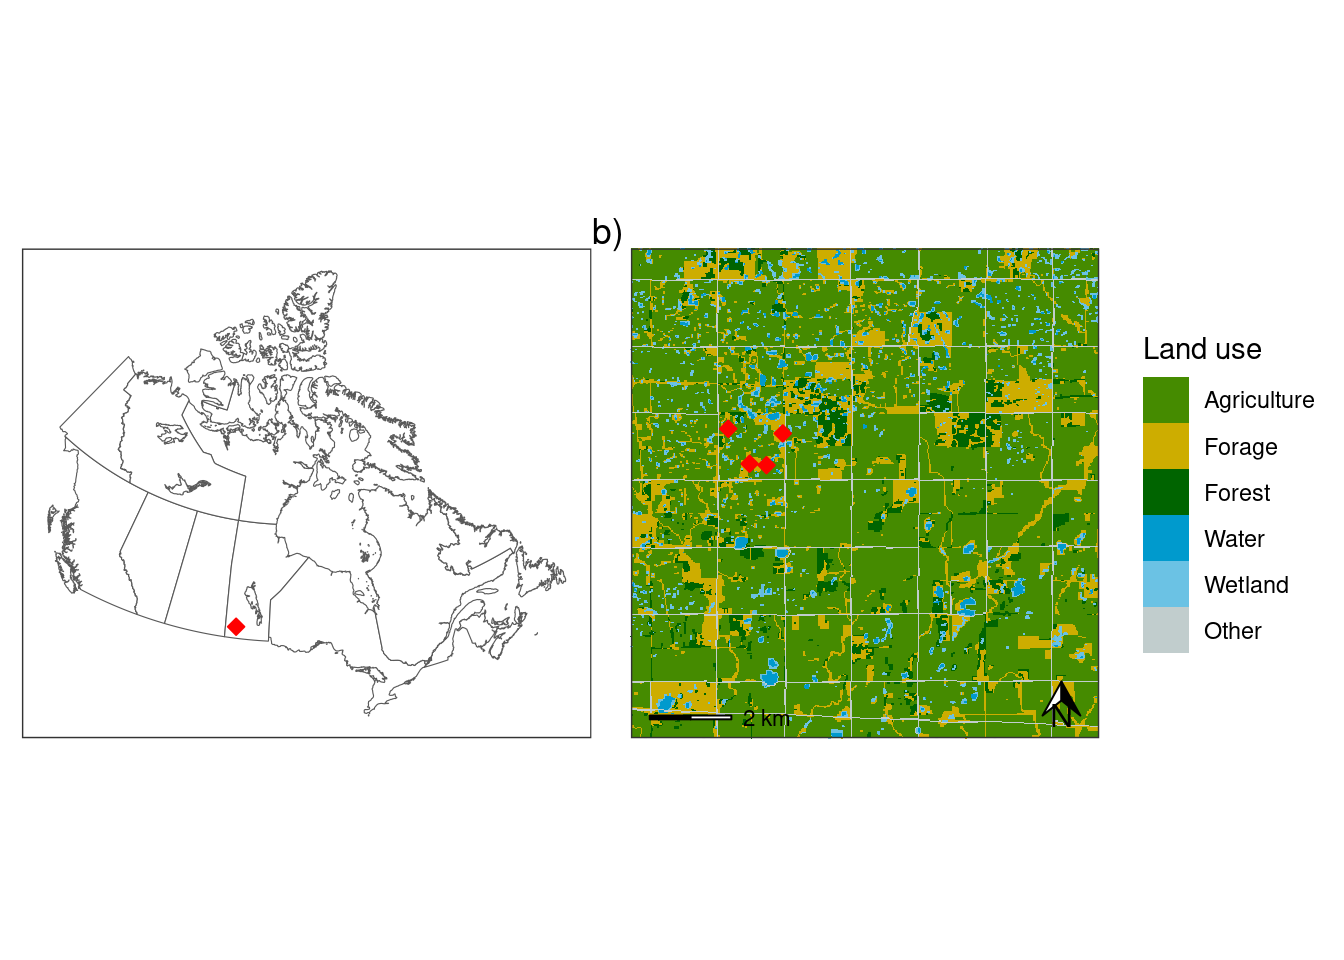
\includegraphics{index_files/figure-latex/notebooks-05_Map-fig-map-output-1.png}

}

\caption{\label{fig-map}Showing a) the study site in southwestern
Manitoba and b) the four riparian areas included in this study and the
regional land use (data from https://mli.gov.mb.ca/).}

\end{figure}%

\textsubscript{Source:
\href{https://alex-koiter.github.io/riparian-grazing-manuscript/notebooks/05_Map-preview.html\#cell-fig-map}{Map
of study area}}

\subsection{Experimental design}\label{experimental-design}

Four riparian areas surrounding permanent wetlands were selected
(Figure~\ref{fig-map}) and were subdivided into four \textasciitilde450
\(m^2\) plots. Within each riparian area each plot was randomly assigned
a treatment. The treatments consisted of a: 1) control, 2) graze, 3)
high density graze, and 4) mow and harvest. The grazing treatments
consisted of a five hour grazing period with the graze treatment having
\textasciitilde3.1-3.5 animal units (AU) per plot and the high density
graze with \textasciitilde11.75-12 AU. For the mowing treatment, the
vegetation was cut to a height of \textasciitilde10cm and the vegetation
manually raked out of the plot. The cattle were rotated daily over four
consecutive days among the four riparian areas and the grazed plots were
fenced on all four sides, including the waters edge, and provided with
supplemental water. Treatments were applied early to mid September,
before the first frost, in three consecutive years (2019-2021)
(\quartosuppfigref{suppfig-weather-plot}) Within each plot three
distinctive sampling zones, or landscape positions, were established,
adjacent to the waters edged (Lower), adjacent to the field/pasture
(Upper), and the mid-point (Mid). To assess the impact of grazing and
mowing, samples were collected in each plot and zone 1-3 days prior and
immediately adjacent 1-3 days following the treatments (including the
control).

\subsection{Sampling and analysis}\label{sampling-and-analysis}

Four types of samples were collected: 1) biomass, 2) litter, 3) organic
layer, and 4) Ah horizon. Using a 0.25 \(m^2\) quadrate, biomass was
collected by cutting the standing live vegetation and litter by raking
the surface and picking up previous years growth. Both the biomass and
litter were dried at 40 \(^\circ C\), weighed, and homogenized using a
blade grinder (\textless1cm). A composite of five soil samples were
collected within the same quadrate as the biomass/litter using a 19 mm
diameter soil probe and were divided into the organic layer and the top
10 cm of the Ah horizon. The organic layer and Ah soil were air-dried,
disaggregated with a mortar and pestle, and passed through a 2-mm sieve.
Additional bulk density samples of both the organic layer and Ah and the
depth of the organic layer were collected in 2023. Daily air temperature
and rainfall data were collected from an onsite station
(\quartosuppfigref{suppfig-weather-plot}) (Manitoba Agriculture, 2023).

Water Extractable Phosphorus (WEP), an environmental soil and vegetation
P test, was used to mimic soil P release to runoff water. Dried and
homogenized samples were extracted by shaking (150 RPM) with deionized
water for one hour at a mass to volume ratio of 1:30 for the biomass and
litter samples (1 g) and 1:15 for the organic and Ah samples (2 g).
Extractions were gravity filtered through a Whatman 42 filter followed
by syringe filtration with a 0.45 \(\mu m\) nylon filter. WEP in the
extract was measured spectrophotometrically by the colorimetric
molybdate--ascorbic acid method (Murphy and Riley, 1962; Sharpley et
al., 2006).

The concentration of WEP in the biomass and litter combined with the
mass of material in collected from the quadrate was used to calculate
the total WEP (\(mg~kg^{-1}\)). Only the change in concentration
(\(mg~kg^{-1}\)) was measured for the organic layer and Ah horizon. The
vertical profile of WEP within the riparian area was assessed using
samples collected before treatments were implemented across the 3-year
study. The total WEP in the organic layer and Ah were estimated using
the bulk density and depth measurements collected in 2023
(Figure~\ref{fig-vertical-wep} b).

\subsection{Statistical analysis}\label{statistical-analysis}

All statistical analysis was undertaken using the R Statistical Software
(v4.3.3), through the RStudio Integrated Development Environment
v2023.12.1.402. Generalized Linear Mixed Models (R package
\texttt{glmmTMB} v1.1.8) were used to investigate the relation between
the change in WEP (before - after treatment) and treatment and riparian
zone for each of the four sources of WEP. Year and riparian area were
included as crossed random factors to control for the variability
between years and riparian areas. Additionally, when investigating the
change in biomass WEP the WEP prior to the treatment was included as a
co-variate the because the magnitude of the difference (i.e., before -
after) is directly related to the amount initially available.

If there were no significant (p \textless0.5) interaction between main
effects the interaction term was removed. When a main effect or
interaction were significant a post-hoc pairwise comparisons with a
Benjamini-Hochberg p value adjustment were used (\texttt{emmeans}
v1.8.9). Model assumptions were assessed using DHARMa residual plots
(\texttt{DHARMa} v0.4.6), main effects were tested for collinearity
(\texttt{performance} v0.10.8.7), and results are presented as type III
ANOVA (\texttt{car} v3.1.2). All plots were created using the R package
\texttt{ggplot2} (v3.5.0).

\section{Results}\label{results}

There is strong vertical stratification in both the concentration and
total WEP (Figure~\ref{fig-vertical-wep}). The median concentration in
the vegetation sources (82.8 - 39.0 \(mg~kg^{-1}\); biomass and litter)
are more than an order of magnitude greater than the soil components
(0.9 - 3.4 \(mg~kg^{-1}\); Ah and organic). The median concentrations
are similar between the upper, mid, and lower positions in the biomass,
organic, and Ah sources. There is a gradient in the median WEP
concentration for the litter where an increase of \textasciitilde20
\(mg~kg^{-1}\) is observed from the upper to lower riparian zone. There
is considerable variability in the WEP concentration in the biomass and
litter sources with interquatile ranges (IQR) of 54.3 and 32.9
\(mg~kg^{-1}\) for the biomass and litter sources, respectively. In
contrast, the IQR for the organic and Ah sources were \textless2.5
\(mg~kg^{-1}\). Overall, in terms of the total amount of WEP, the top 10
cm of the Ah horizon is the largest source of WEP (42.5 \(mg~m^{-2}\))
followed by the biomass (26.3 \(mg~m^{-2}\)), organic layer (14.3
\(mg~m^{-2}\)), and lastly the litter (13.7 \(mg~m^{-2}\)). In contrast
to the concentration the total WEP does show an impact of the riparian
zone. For the biomass and litter sources the lower riparian zones had
greater amounts of WEP whereas the organic and Ah sources had greater
amount of WEP in the upper riparian zones. The amount of variability is
greatest in the Ah (IQR = 32.0 \(mg~kg^{-1}\)) and biomass (IQR = 23.3
\(mg~kg^{-1}\)) sources. The variability of the other two sources were
similar with IQRS of 15.6 and 14.3 \(mg~kg^{-1}\) for the litter and
organic layer, respectively.

\begin{figure}[H]

\centering{

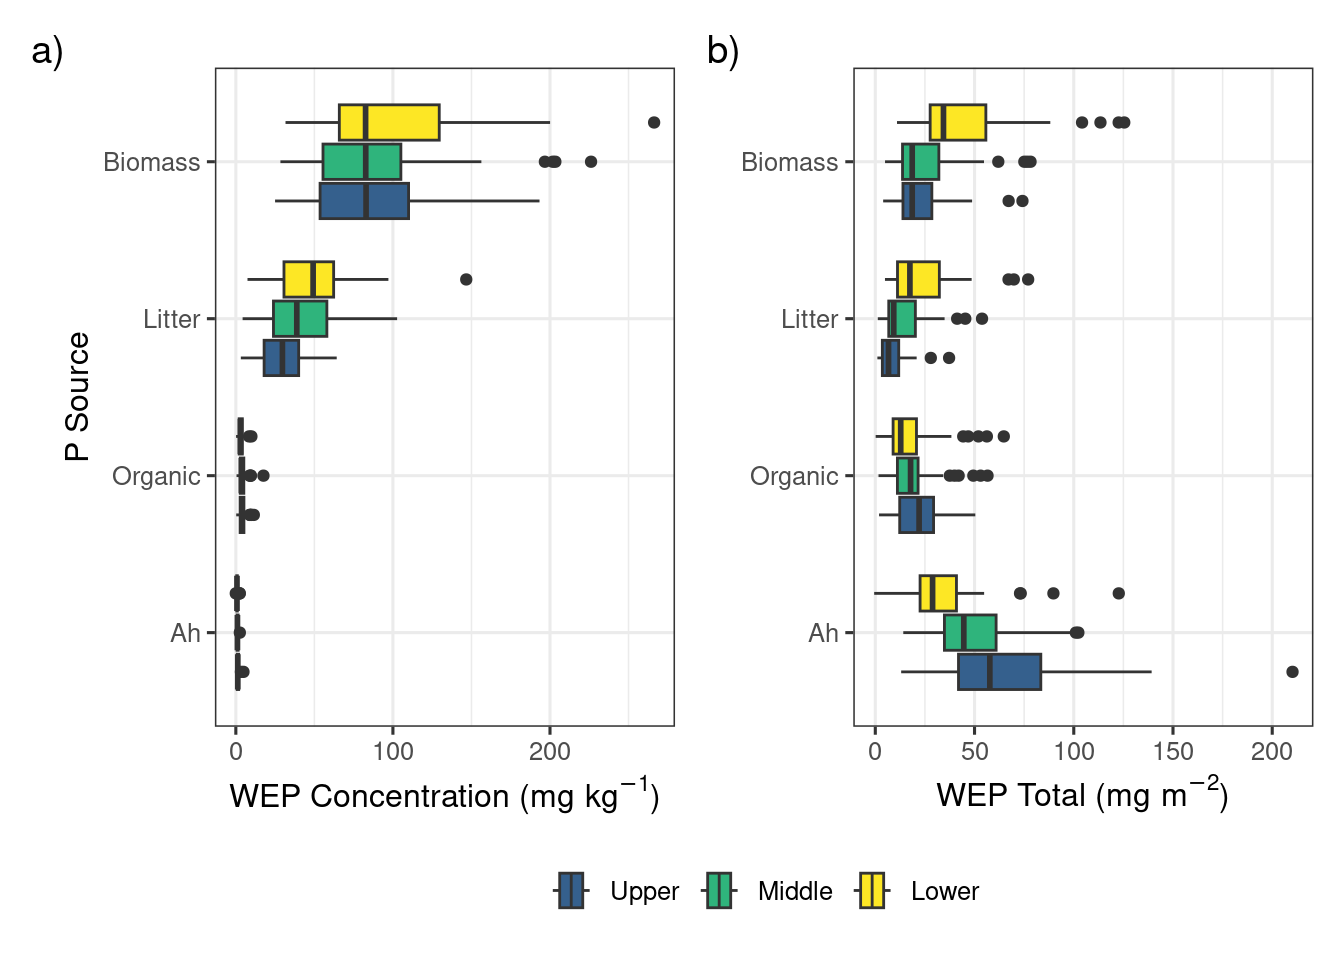
\includegraphics{index_files/figure-latex/notebooks-04_Vertical_profile-fig-vertical-wep-output-2.png}

}

\caption{\label{fig-vertical-wep}Vertical and longitudinal profiles of
a) WEP concentration and b) WEP content in the riparian areas prior to
grazing and mowing treatments.}

\end{figure}%

\textsubscript{Source:
\href{https://alex-koiter.github.io/riparian-grazing-manuscript/notebooks/04_Vertical_profile-preview.html\#cell-fig-vertical-WEP}{Vertical
profile of WEP}}

Both the high density grazing and mowing treatments significantly
(p\textless0.05) reduced the total amount of the biomass WEP compared to
the control and graze treatments (Figure~\ref{fig-vegetation-wep} a).
The mowing and high density grazing reduced the average WEP amount by
7.4 and 4.2 \(mg~m^{-2}\) relative to the control, respectively. The
reduction in biomass WEP was significantly (p\textless0.05) greater in
the lower zones as compared to the upper and mid zones
(Figure~\ref{fig-vegetation-wep} b) with a difference in average WEP of
10.2 \(mg~m^{-2}\) between the lower and upper zones of the riparian
area.

\begin{figure}[H]

\centering{

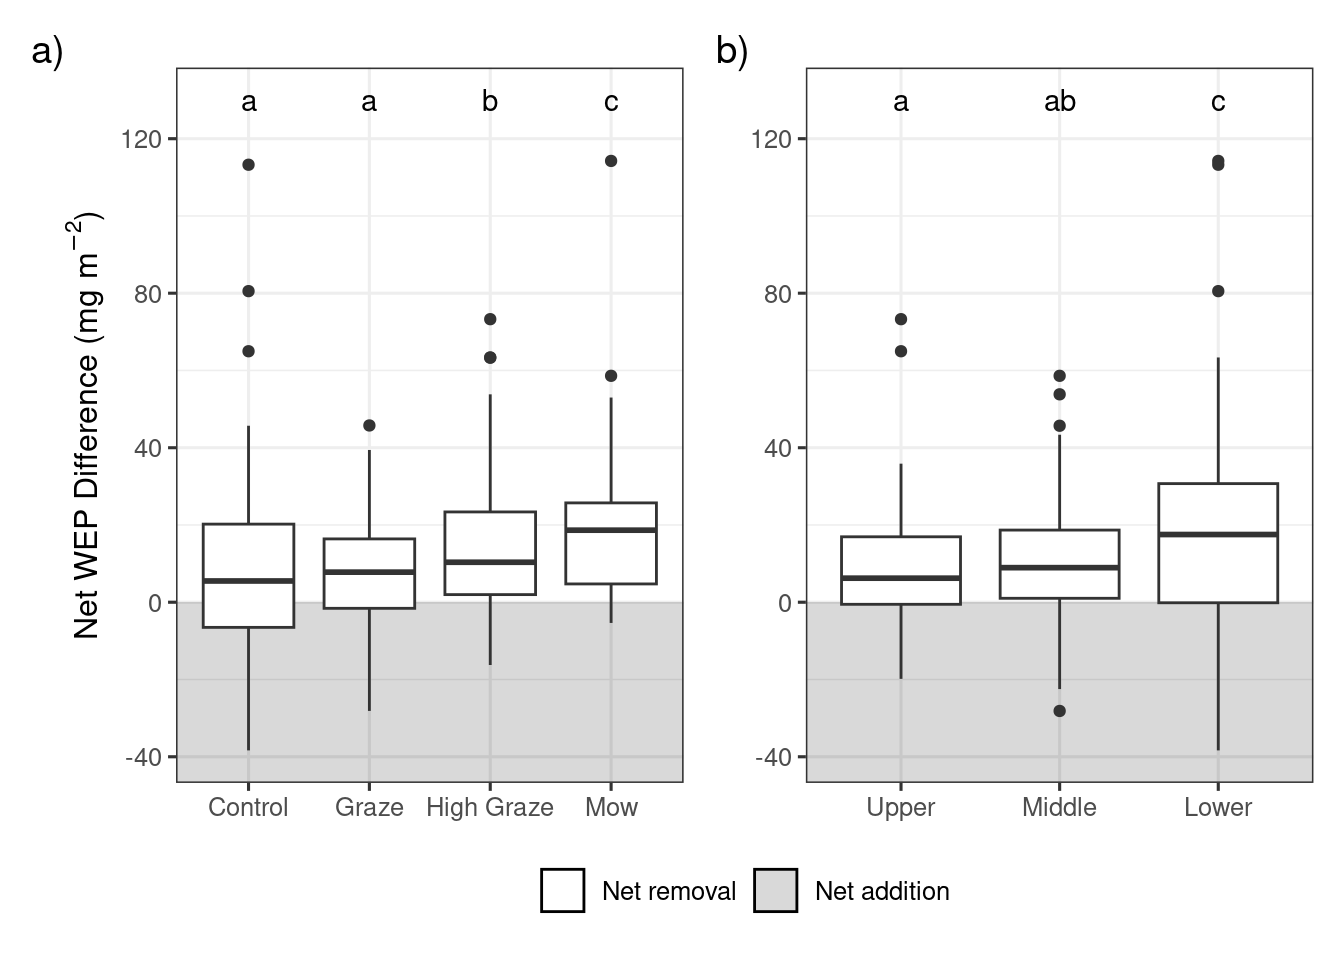
\includegraphics{index_files/figure-latex/notebooks-01_Biomass_analysis-fig-vegetation-wep-output-2.png}

}

\caption{\label{fig-vegetation-wep}Change in riparian biomass WEP
following grazing or mowing in each riparian zone. Within each plot
significant differences (p\textless0.05) between treatments or riparian
zones are denoted with different letters.}

\end{figure}%

\textsubscript{Source:
\href{https://alex-koiter.github.io/riparian-grazing-manuscript/notebooks/01_Biomass_analysis-preview.html\#cell-fig-vegetation-WEP}{Riparian
vegetation WEP in response to grazing}}

There were no significant impacts of either treatment or riparian zone
on the amount of litter WEP (Figure~\ref{fig-litter-wep}). The ANOVA
detected a significant (p = 0.04) effect of treatment on the WEP
concentration in the organic layer; however, no significant differences
were observed between any post-hoc pairwise comparisons
(Figure~\ref{fig-organic-wep}). Lastly, there was no significant effect
of treatment or riparian zone in the concentration of WEP in the top 10
cm of the Ah horizon (Figure~\ref{fig-soil-wep}). There was considerable
variation across all treatments and riparian zones in all four sources
of P. This high variability in WEP amount/concentration is best
reflected in the control treatment were the expected difference is 0 but
there were measured WEP losses and gains despite no treatment being
applied.

\begin{figure}[H]

\centering{

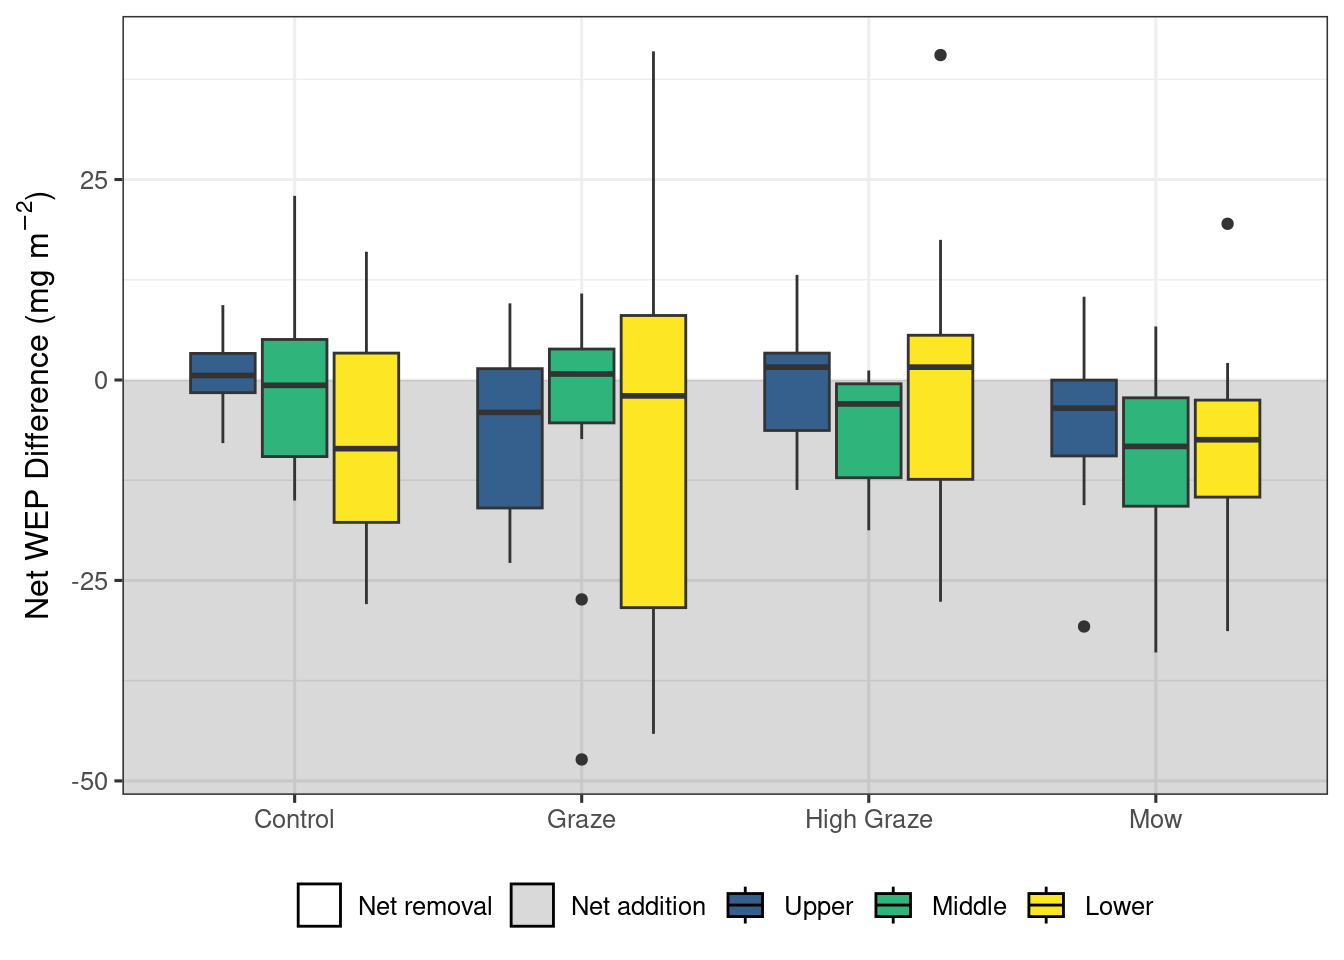
\includegraphics{index_files/figure-latex/notebooks-02_Litter_analysis-fig-litter-wep-output-2.png}

}

\caption{\label{fig-litter-wep}Change in riparian litter WEP following
grazing or mowing in each of the riparian zones. No significant effect
of treatment or riparian zone on the litter WEP content was detected}

\end{figure}%

\textsubscript{Source:
\href{https://alex-koiter.github.io/riparian-grazing-manuscript/notebooks/02_Litter_analysis-preview.html\#cell-fig-litter-WEP}{Riparian
litter WEP in response to grazing}}

\begin{figure}[H]

\centering{

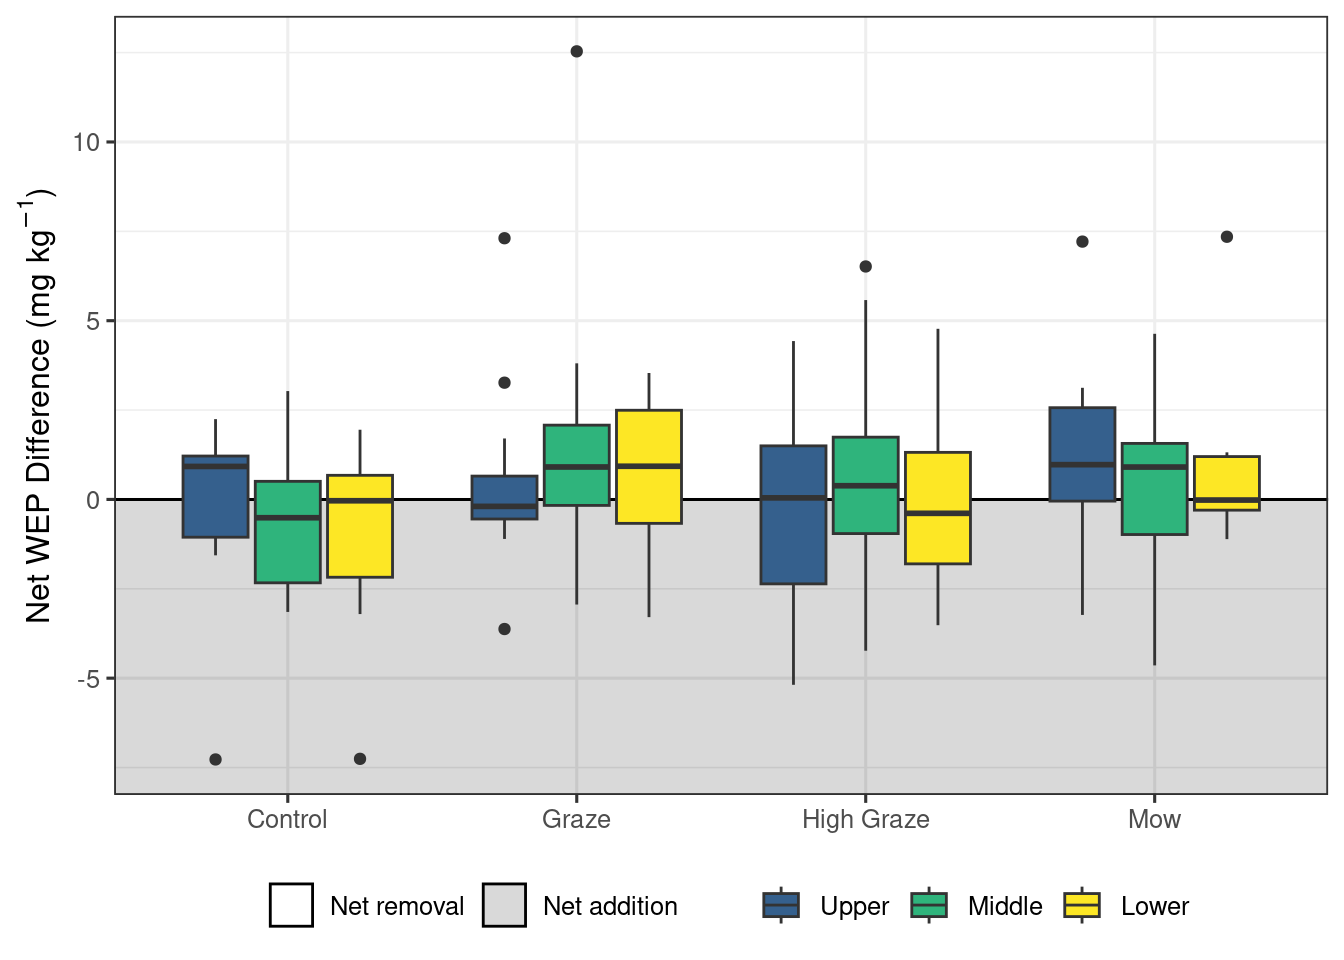
\includegraphics{index_files/figure-latex/notebooks-03_Soils_analysis-fig-organic-wep-output-1.png}

}

\caption{\label{fig-organic-wep}Change in riparian organic layer WEP
concentration following grazing or mowing in each of the riparian zones.
A significant effect of treatment was detected; however, the post-hoc
analysis was not able to detect any significant (p \textless{} 0.05)
pairwise contrasts.}

\end{figure}%

\textsubscript{Source:
\href{https://alex-koiter.github.io/riparian-grazing-manuscript/notebooks/03_Soils_analysis-preview.html\#cell-fig-organic-WEP}{Riparian
organic and mineral soil WEP in response to grazing}}

\begin{figure}[H]

\centering{

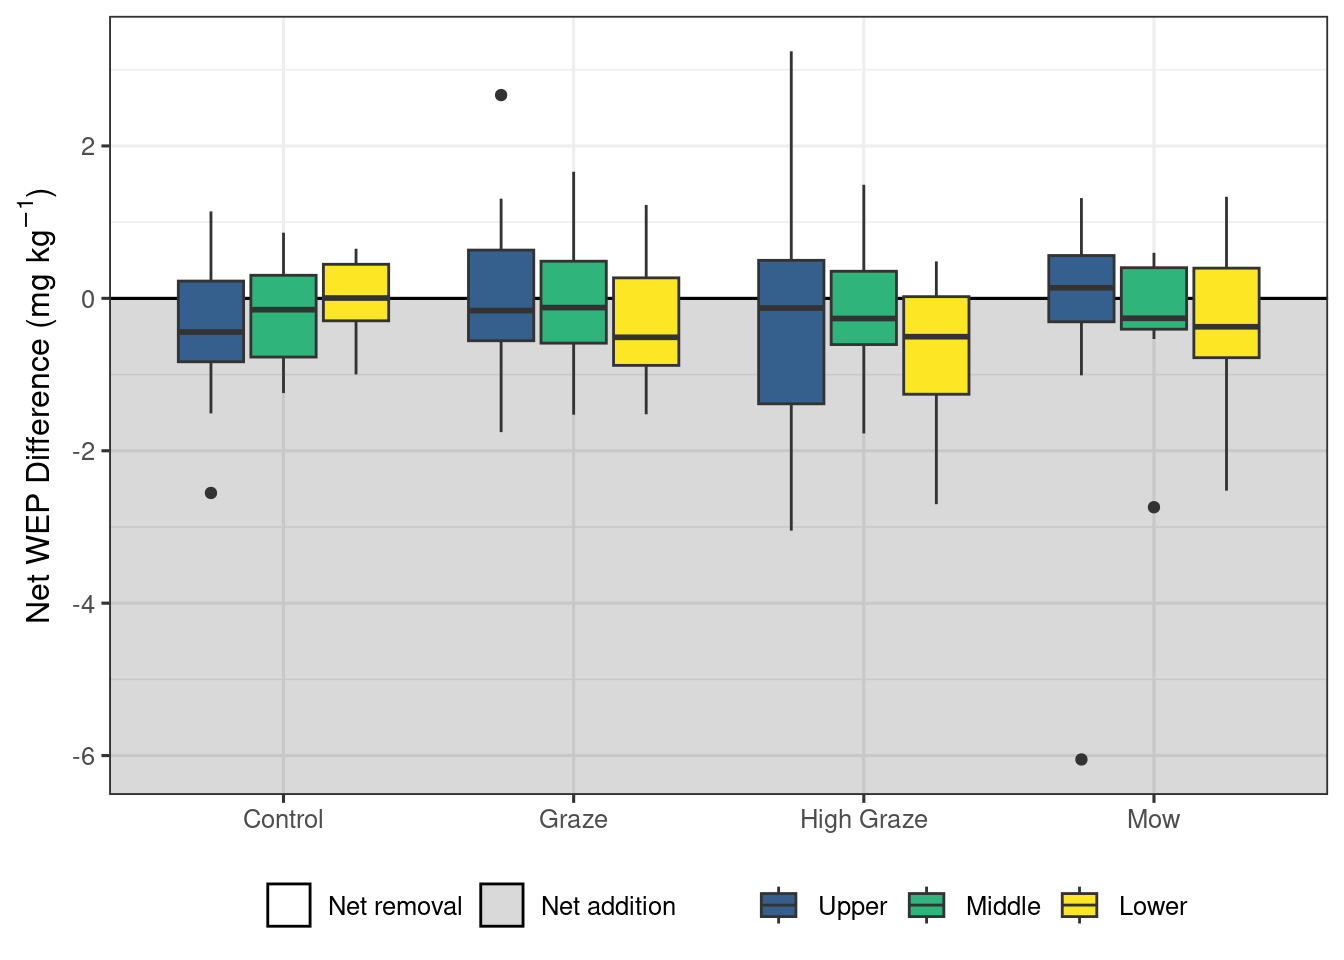
\includegraphics{index_files/figure-latex/notebooks-03_Soils_analysis-fig-soil-wep-output-1.png}

}

\caption{\label{fig-soil-wep}Change in riparian Ah layer (0-10cm) WEP
concentration following grazing or mowing in each of the riparian zones.
No significant effect of treatment or zone was detected.}

\end{figure}%

\textsubscript{Source:
\href{https://alex-koiter.github.io/riparian-grazing-manuscript/notebooks/03_Soils_analysis-preview.html\#cell-fig-soil-WEP}{Riparian
organic and mineral soil WEP in response to grazing}}

\section{Discussion}\label{discussion}

The vertical profile of WEP in riparian areas
(Figure~\ref{fig-vertical-wep}) observed in this study supports the
concept that a soil test P alone is likely missing a large proportion of
the near-surface P that can be potentially lost during the spring
snowmelt (Liu et al., 2019a; b; Cober et al., 2019). The substantial
proportion of WEP above the soil surface provides evidence that that
managing the biomass in riparian areas in the autumn may reduce the
contribution of P lost directly from this area during the spring. The
measured WEP in this study may underestimate the total WEP during the
spring snowmelt as the as repeated and severity of FTC on WEP was not
characterized (Roberson et al., 2007; Lozier and Macrae, 2017).
Additionally, harvesting of this biomass results in an export of P which
can maintain or enhance the buffering or storage capacity of P derived
from upslope sources further improving downstream water quality (Kelly
et al., 2007; Hille et al., 2019). The longitudinal gradient of WEP
shows an inverted symmetry where the biomass WEP is largest near the
waters edge and the Ah soil WEP is larger in the upper zone adjacent to
the fields (Figure~\ref{fig-vertical-wep} b). The high soil water
content in the lower zone creates conditions that favour high biomass
production (\quartosuppfigref{suppfig-bd-plot}) coupled with high
biomass WEP concentrations (Figure~\ref{fig-vertical-wep} a) results in
a considerable source of P. The higher amount of WEP in the Ah soil in
the upper zone of the riparian area is due to the higher bulk density
(\quartosuppfigref{suppfig-bd-plot}) and higher WEP concentration
(Figure~\ref{fig-vertical-wep} a). The higher bulk density is most
likely due to the lower soil organic matter content and the higher WEP
concentration may be related to the interception of P-rich runoff from
upslope areas (Tomer et al., 2007). Understanding and quantifying the
sources and patterns of P within riparian areas is a key part of
assessing the risk of P loss and designing effective management plans
(Reid et al., 2018).

The results of this study suggest that short-term autumn high density
grazing may be a potential management tool that can reduce the amount of
P lost directly from the riparian area (Figure~\ref{fig-vegetation-wep}
a). In addition to managing P loss, grazing riparian areas can also
provide an important source of forage, particularly during drought.
Mechanized harvesting of biomass will also achieve this reduction in P
loss (Figure~\ref{fig-vegetation-wep} a) if the landscape and soil
conditions are favourable. Despite the cycling of nutrients by the
removal of P through grazing of biomass
(Figure~\ref{fig-vegetation-wep}) and the deposition through excretion
no differences were detected in the litter and Ah sources of P
(Figure~\ref{fig-litter-wep}, and \ref{fig-soil-wep}). The ANOVA did
detect a significant effect of treatment on the organic layer WEP;
however, the pairwise comparisons was not able to detect any significant
differences and the exact nature of the impact of the treatments remains
unclear. The ability to detect changes in the WEP sources in riparian
areas is difficult due to both the inherent and post-grazing treatment
spatial variability. Even within the control plots, both net addition
and removal of WEP were measured and in many cases the amount of
variability was similar across treatments. This inherent variability
(i.e., pre-grazing) is a result of a combination of hydrological factors
like ground water fluctuations, soil attributes such as texture,
ecological dynamics involving plant community composition, and
anthropogenic influences like historic land management practices
(McClain et al., 2003; Vidon et al., 2010). Post-grazing treatment, the
added urine and manure creates additional hotspots of P that may carry
forward to subsequent years (Subedi et al., 2020; Donohoe et al., 2021).
The single 0.25 \(m^2\) sampling quadrate within each riparian zone may
have been insufficient to capture the spatial variability. Therefore,
larger, composite, and/or several sampling locations within each zone is
recommended. Appropriate sampling design becomes more important as the
scale of observation of similar research increases to the farm scale so
will the amount and source of variability. As the scope of research is
expanded to the farm level, the importance of using an appropriate
sampling design becomes increasingly critical (Hale et al., 2014).

Autumn was selected for the mowing and grazing treatments for three
reasons. First was to reduce the amount of biomass P available that can
contribute to the P loss during the spring snowmelt. Secondly, the drier
soil conditions reduced the amount of pugging and soil compaction which
limits the disruption of soil structure and damage to plants (Batey,
2009). Lastly, the prairie potholes and associated riparian areas are
important breeding habitat for migratory birds and late season grazing
may reduce the ecological impact (Stanley and Knopf, 2002). However, the
type of grazing system (timing, stocking rate and density etc.) may
impact habitat quality and breeding success (Carnochan et al., 2018;
Hansen et al., 2019; Kraft et al., 2021). Corridor fencing at the waters
edge and alternative water sources were used in this study to limit
livestock access to prevent bank erosion and protect water quality
(e.g., direct deposition) (Dauwalter et al., 2018). Scaling this up to
the farm level will be expensive (fencing infrastructure) (Aarons et
al.,) and time consuming (short-term grazing), especially in prairie
pothole region were there are numerous and small riparian areas
(Manitoba Agriculture, 2024). The long-term impacts of repeated grazing
of riparian areas also needs to be considered. From a nutrient loss
reduction perspective, a shift in the magnitude of the sources of P
could be expected as less biomass is available to be added to the litter
source, which in turn effects the organic layer and Ah sources of P. The
regular inclusion of cattle will also introduce new manure source of P
which can spatially redistribute P, and initially be more water soluble
and readily transported (Franzluebbers et al., 2019). Grazing can also
reduce the litter layer through trampling increasing the soil-vegetation
contact speeding up the decomposition process. These changes in biomass
and litter quantities may result in changes to habitat structure.
Understanding how of forage management directly impacts both the plant
and soil P dynamics is important for understanding both the agronomic
and environmental P considerations (Subedi et al., 2020).

\section{Conclusion}\label{conclusion}

Biomass and litter are significant sources of near surface WEP in
riparian areas that historically have been disregarded as important.
Management of the biomass prior to the onset of winter conditions in
cold climates has the potential to reduce the amount of P directly lost
during the spring snowmelt and maintain or enhance the nutrient
buffering capacity. The results from this experiment demonstrated that
short-term high density cattle grazing and mowing both resulted in a
reduction in the amount of biomass WEP, particularly in the lower
riparian zones. The grazing and mowing treatments had no detectable
effect on the other three near-surface sources of WEP. However,
detecting changes in the near-surface sources of WEP is challenging due
to high spatial variability.

Comparatively less riparian research has occurred in landscapes that
experience a cold climate with strong temperature seasonality (e.g.,
Canadian prairies). In these regions the runoff and nutrient losses
occur predominately during the spring snowmelt period. The repeated FTC
of the vegetation and soils increase the potential P losses during this
key time. Continued research to identify, quantify, and manage these
sources of P to improve water quality remains a priority. In addition to
water quality improvement, the development of riparian management
strategies should also prioritize the protection other ecological goods
and services and recognize these areas as an integral part of the farm.

\section*{Acknowledgements}\label{acknowledgements}
\addcontentsline{toc}{section}{Acknowledgements}

This project was undertaken with the financial support of the Government
of Canada through the federal Department of Environment and Climate
Change and a Lake Winnipeg Basin Program grant awarded to the Manitoba
Association of Watersheds. Additional research funding was provided
through a Brandon University Research Committee grant awarded to AK.
Thank you to A. Avila, M. Luna, C Sobchuk, and A. Tan for all the help
with lab and field work. Special thanks to the Manitoba Beef and Forage
Initiatives research farm staff for the use of their facilities and
managing the cattle grazing and mowing treatments. Lastly, thank you to
R. Canart and M. Elsinger for helping to develop the experimental
design.

\section*{Data availability}\label{data-availability}
\addcontentsline{toc}{section}{Data availability}

Data and source code for analysis and manuscript available on GitHub:
\url{https://github.com/alex-koiter/riparian-grazing-manuscript}

\section*{Conflict of interest
statement}\label{conflict-of-interest-statement}
\addcontentsline{toc}{section}{Conflict of interest statement}

The authors have no competing interests to declare that are relevant to
the content of this article.

\section*{Author contributions}\label{author-contributions}
\addcontentsline{toc}{section}{Author contributions}

The authors confirm contribution to the paper as follows: study
conception and design: A. Koiter; data collection: T. Malone; analysis
and interpretation of results: A. Koiter; draft manuscript preparation:
A. Koiter and T. Malone. All authors reviewed the results and approved
the final version of the manuscript.

\section*{References}\label{references}
\addcontentsline{toc}{section}{References}

\phantomsection\label{refs}
\begin{CSLReferences}{1}{1}
\vspace{1em}

\bibitem[\citeproctext]{ref-aarons2013}
Aarons, S.R., A.R. Melland, and L. Dorling. Dairy farm impacts of
fencing riparian land: Pasture production and farm productivity. Journal
of Environmental Management 130: 255--266. doi:
\href{https://doi.org/10.1016/j.jenvman.2013.08.060}{10.1016/j.jenvman.2013.08.060}.

\bibitem[\citeproctext]{ref-batey2009}
Batey, Tom. 2009. Soil compaction and soil management {\textendash} a
review. Soil Use and Management 25(4): 335--345. doi:
\href{https://doi.org/10.1111/j.1475-2743.2009.00236.x}{10.1111/j.1475-2743.2009.00236.x}.

\bibitem[\citeproctext]{ref-beck2018}
Beck, H.E., N.E. Zimmermann, T.R. McVicar, N. Vergopolan, A. Berg, et
al. 2018. Present and future Köppen-Geiger climate classification maps
at 1-km resolution. Scientific Data 5(1): 180214. doi:
\href{https://doi.org/10.1038/sdata.2018.214}{10.1038/sdata.2018.214}.

\bibitem[\citeproctext]{ref-borin2005}
Borin, Maurizio., Monica. Vianello, Francesco. Morari, and Giuseppe.
Zanin. 2005. Effectiveness of buffer strips in removing pollutants in
runoff from a cultivated field in north-east italy. Agriculture,
Ecosystems \& Environment 105(1): 101114. doi:
\href{https://doi.org/doi:10.1016/j.agee.2004.05.011}{doi:10.1016/j.agee.2004.05.011}.

\bibitem[\citeproctext]{ref-carlyle2001}
Carlyle, G.C., and A.R. Hill. 2001. Groundwater phosphate dynamics in a
river riparian zone: Effects of hydrologic flowpaths, lithology and
redox chemistry. Journal of Hydrology 247(3): 151--168. doi:
\href{https://doi.org/10.1016/S0022-1694(01)00375-4}{10.1016/S0022-1694(01)00375-4}.

\bibitem[\citeproctext]{ref-carnochan2018}
Carnochan, S.J., C.C. De Ruyck, and N. Koper. 2018. Effects of
twice-over rotational grazing on songbird nesting success in years with
and without flooding. Rangeland Ecology \& Management 71(6): 776--782.
doi:
\href{https://doi.org/10.1016/j.rama.2018.04.013}{10.1016/j.rama.2018.04.013}.

\bibitem[\citeproctext]{ref-cober2019}
Cober, J.R., M.L. Macrae, and L.L. Van Eerd. 2019. Winter phosphorus
release from cover crops and linkages with runoff chemistry. Journal of
Environmental Quality 48(4): 907--914. doi:
\href{https://doi.org/10.2134/jeq2018.08.0307}{10.2134/jeq2018.08.0307}.

\bibitem[\citeproctext]{ref-cole2015}
Cole, L.J., S. Brocklehurst, D. Robertson, W. Harrison, and D.I.
McCracken. 2015. Riparian buffer strips: Their role in the conservation
of insect pollinators in intensive grassland systems. Agriculture,
Ecosystems \& Environment 211: 207--220. doi:
\href{https://doi.org/10.1016/j.agee.2015.06.012}{10.1016/j.agee.2015.06.012}.

\bibitem[\citeproctext]{ref-cole2020}
Cole, L.J., J. Stockan, and R. Helliwell. 2020. Managing riparian buffer
strips to optimise ecosystem services: A review. Agriculture, Ecosystems
\& Environment 296: 106891. doi:
\href{https://doi.org/10.1016/j.agee.2020.106891}{10.1016/j.agee.2020.106891}.

\bibitem[\citeproctext]{ref-dauwalter2018}
Dauwalter, D.C., K.A. Fesenmyer, S.W. Miller, and T. Porter. 2018.
Response of Riparian Vegetation, Instream Habitat, and Aquatic Biota to
Riparian Grazing Exclosures. North American Journal of Fisheries
Management 38(5): 1187--1200. doi:
\href{https://doi.org/10.1002/nafm.10224}{10.1002/nafm.10224}.

\bibitem[\citeproctext]{ref-dillaha1989}
Dillaha, T.A., R.B. Reneau, S. Mostaghimi, and D. Lee. 1989. Vegetative
filter strips for agricultural nonpoint source pollution control.
Transactions of the American Society of Agricultural Engineers 32(2):
513519. doi:
\href{https://doi.org/10.13031/2013.31033}{10.13031/2013.31033}.

\bibitem[\citeproctext]{ref-donohoe2021}
Donohoe, G., D. Flaten, F. Omonijo, and K. Ominski. 2021. Short-term
impacts of winter bale grazing beef cows on forage production and soil
nutrient status in the eastern canadian prairies. Canadian Journal of
Soil Science 101(4): 717--733. doi:
\href{https://doi.org/10.1139/cjss-2021-0028}{10.1139/cjss-2021-0028}.

\bibitem[\citeproctext]{ref-dorioz2006}
Dorioz, J.M., D. Wang, J. Poulenard, and D. Trevisan. 2006. The effect
of grass buffer strips on phosphorus dynamics - a critical review and
synthesis as a basis for application in agricultural landscapes in
france. Agriculture, Ecosystems \& Environment 117(1): 4--21. doi:
\href{https://doi.org/10.1016/j.agee.2006.03.029}{10.1016/j.agee.2006.03.029}.

\bibitem[\citeproctext]{ref-elliott2013}
Elliott, J. 2013. Evaluating the potential contribution of vegetation as
a nutrient source in snowmelt runoff. Canadian Journal of Soil Science
93(4): 435--443. doi:
\href{https://doi.org/10.4141/cjss2012-050}{10.4141/cjss2012-050}.

\bibitem[\citeproctext]{ref-environmentandclimatechangecanada2024}
Environment, and Climate Change Canada. 2024. Canadian Climate Normals.
\url{https://climate.weather.gc.ca/climate_normals/index_e.html}.

\bibitem[\citeproctext]{ref-fitch2003}
Fitch, L., B. Adams, and K. O'Shaughnessy. 2003. Caring for the green
zone: Riparian areas and grazing management. 3rd ed. Cows; Fish Program,
Lethbridge, Alberta.

\bibitem[\citeproctext]{ref-forio2020}
Forio, M.A.E., N. De Troyer, K. Lock, F. Witing, L. Baert, et al. 2020.
Small Patches of Riparian Woody Vegetation Enhance Biodiversity of
Invertebrates. Water 12(11): 3070. doi:
\href{https://doi.org/10.3390/w12113070}{10.3390/w12113070}.

\bibitem[\citeproctext]{ref-franzluebbers2019}
Franzluebbers, A.J., M.H. Poore, S.R. Freeman, and J.R. Rogers. 2019.
Soil-surface nutrient distributions in grazed pastures of North
Carolina. Journal of Soil and Water Conservation 74(6): 571--583. doi:
\href{https://doi.org/10.2489/jswc.74.6.571}{10.2489/jswc.74.6.571}.

\bibitem[\citeproctext]{ref-gregory1991}
Gregory, S.V., F.J. Swanson, W.A. McKee, and K.W. Cummins. 1991. An
ecosystem perspective of riparian zones. BioScience 41(8): 540551. doi:
\href{https://doi.org/10.2307/1311607}{10.2307/1311607}.

\bibitem[\citeproctext]{ref-habibiandehkordi2019}
Habibiandehkordi, R., D.A. Lobb, P.N. Owens, and D.N. Flaten. 2019.
Effectiveness of vegetated buffer strips in controlling legacy
phosphorus exports from agricultural land. Journal of Environmental
Quality 48(2): 314--321. doi:
\href{https://doi.org/10.2134/jeq2018.04.0129}{10.2134/jeq2018.04.0129}.

\bibitem[\citeproctext]{ref-habibiandehkordi2017}
Habibiandehkordi, R., D.A. Lobb, S.C. Sheppard, D.N. Flaten, and P.N.
Owens. 2017. Uncertainties in vegetated buffer strip function in
controlling phosphorus export from agricultural land in the canadian
prairies. Environmental Science and Pollution Research 24(22):
18372--18382. doi:
\href{https://doi.org/10.1007/s11356-017-9406-6}{10.1007/s11356-017-9406-6}.

\bibitem[\citeproctext]{ref-hale2014}
Hale, R., P. Reich, T. Daniel, P.S. Lake, and T.R. Cavagnaro. 2014.
Scales that matter: Guiding effective monitoring of soil properties in
restored riparian zones. Geoderma 228-229: 173--181. doi:
\href{https://doi.org/10.1016/j.geoderma.2013.09.019}{10.1016/j.geoderma.2013.09.019}.

\bibitem[\citeproctext]{ref-hansen2019}
Hansen, B.D., H.S. Fraser, and C.S. Jones. 2019. Livestock grazing
effects on riparian bird breeding behaviour in agricultural landscapes.
Agriculture, Ecosystems \& Environment 270-271: 93--102. doi:
\href{https://doi.org/10.1016/j.agee.2018.10.016}{10.1016/j.agee.2018.10.016}.

\bibitem[\citeproctext]{ref-hille2019}
Hille, S., D. Graeber, B. Kronvang, G.H. Rubæk, N. Onnen, et al. 2019.
Management Options to Reduce Phosphorus Leaching from Vegetated Buffer
Strips. Journal of Environmental Quality 48(2): 322--329. doi:
\href{https://doi.org/10.2134/jeq2018.01.0042}{10.2134/jeq2018.01.0042}.

\bibitem[\citeproctext]{ref-kelly2007}
Kelly, J.M., J.L. Kovar, R. Sokolowsky, and T.B. Moorman. 2007.
Phosphorus uptake during four years by different vegetative cover types
in a riparian buffer. Nutrient Cycling in Agroecosystems 78(3):
239--251. doi:
\href{https://doi.org/10.1007/s10705-007-9088-4}{10.1007/s10705-007-9088-4}.

\bibitem[\citeproctext]{ref-kieta2019}
Kieta, K.A., and P.N. Owens. 2019. Phosphorus release from shoots of
phleum pretense l. After repeated freeze-thaw cycles and harvests.
Ecological Engineering 127: 204--211. doi:
\href{https://doi.org/10.1016/j.ecoleng.2018.11.024}{10.1016/j.ecoleng.2018.11.024}.

\bibitem[\citeproctext]{ref-kieta2018}
Kieta, K.A., P.N. Owens, D.A. Lobb, J.A. Vanrobaeys, and D.N. Flaten.
2018. Phosphorus dynamics in vegetated buffer strips in cold climates: A
review. Environmental Reviews 26(3): 255--272. doi:
\href{https://doi.org/10.1139/er-2017-0077}{10.1139/er-2017-0077}.

\bibitem[\citeproctext]{ref-kraft2021}
Kraft, J.D., D.A. Haukos, M.R. Bain, M.B. Rice, S. Robinson, et al.
2021. Using Grazing to Manage Herbaceous Structure for a
Heterogeneity-Dependent Bird. The Journal of Wildlife Management 85(2):
354--368. doi:
\href{https://doi.org/10.1002/jwmg.21984}{10.1002/jwmg.21984}.

\bibitem[\citeproctext]{ref-krall2023}
Krall, M., and P. Roni. 2023. Effects of livestock exclusion on stream
habitat and aquatic biota: A review and recommendations for
implementation and monitoring. North American Journal of Fisheries
Management 43(2): 476--504. doi:
\href{https://doi.org/10.1002/nafm.10863}{10.1002/nafm.10863}.

\bibitem[\citeproctext]{ref-lacas2005}
Lacas, J.-G., M. Voltz, V. Gouy, N. Carluer, and J.-J. Gril. 2005. Using
grassed strips to limit pesticide transfer to surface water: A review.
Agronomy for Sustainable Development 25(2): 253--266. doi:
\href{https://doi.org/10.1051/agro:2005001}{10.1051/agro:2005001}.

\bibitem[\citeproctext]{ref-liu2019}
Liu, J., H.M. Baulch, M.L. Macrae, H.F. Wilson, J.A. Elliott, et al.
2019a. Agricultural water quality in cold climates: processes, drivers,
management options, and research needs. Journal of Environmental Quality
48(4): 792--802. doi:
\href{https://doi.org/10.2134/jeq2019.05.0220}{10.2134/jeq2019.05.0220}.

\bibitem[\citeproctext]{ref-liu2019a}
Liu, J., M.L. Macrae, J.A. Elliott, H.M. Baulch, H.F. Wilson, et al.
2019b. Impacts of cover crops and crop residues on phosphorus losses in
cold climates: a review. Journal of Environmental Quality 48(4):
850--868. doi:
\href{https://doi.org/10.2134/jeq2019.03.0119}{10.2134/jeq2019.03.0119}.

\bibitem[\citeproctext]{ref-lozier2017}
Lozier, T.M., and M.L. Macrae. 2017. Potential phosphorus mobilization
from above-soil winter vegetation assessed from laboratory water
extractions following freeze{\textendash}thaw cycles. Canadian Water
Resources Journal 42(3): 276--288. doi:
\href{https://doi.org/10.1080/07011784.2017.1331140}{10.1080/07011784.2017.1331140}.

\bibitem[\citeproctext]{ref-luther2008}
Luther, D., J. Hilty, J. Weiss, C. Cornwall, M. Wipf, et al. 2008.
Assessing the impact of local habitat variables and landscape context on
riparian birds in agricultural, urbanized, and native landscapes.
Biodiversity and Conservation 17(8): 1923--1935. doi:
\href{https://doi.org/10.1007/s10531-008-9332-5}{10.1007/s10531-008-9332-5}.

\bibitem[\citeproctext]{ref-lyu2021}
Lyu, C., X. Li, P. Yuan, Y. Song, H. Gao, et al. 2021. Nitrogen
retention effect of riparian zones in agricultural areas: A
meta-analysis. Journal of Cleaner Production 315: 128143. doi:
\href{https://doi.org/10.1016/j.jclepro.2021.128143}{10.1016/j.jclepro.2021.128143}.

\bibitem[\citeproctext]{ref-manitobaagriculture2023}
Manitoba Agriculture. 2023. Manitoba agriculture weather program.
\url{https://www.gov.mb.ca/agriculture/weather/manitoba-ag-weather.html}.

\bibitem[\citeproctext]{ref-manitobaagriculture2024}
Manitoba Agriculture. 2024. Agriculture rotational grazing.
\url{https://www.gov.mb.ca/agriculture/}.

\bibitem[\citeproctext]{ref-manitobabeefforageinitiatives2024}
Manitoba Beef \& Forage Initiatives. 2024. MBFI farm stations.
\url{https://www.mbfi.ca/farm-station}.

\bibitem[\citeproctext]{ref-mcclain2003}
McClain, M.E., E.W. Boyer, C.L. Dent, S.E. Gergel, N.B. Grimm, et al.
2003. Biogeochemical hot spots and hot moments at the interface of
terrestrial and aquatic ecosystems. Ecosystems 6(4): 301312. doi:
\href{https://doi.org/10.1007/s10021-003-0161-9}{10.1007/s10021-003-0161-9}.

\bibitem[\citeproctext]{ref-mcguire2010}
McGuire, K.J., and J.J. McDonnell. 2010. Hydrological connectivity of
hillslopes and streams: Characteristic time scales and nonlinearities.
Water Resources Research 46(10): W10543. doi:
\href{https://doi.org/10.1029/2010WR009341}{10.1029/2010WR009341}.

\bibitem[\citeproctext]{ref-montgomery1996}
Montgomery, G. 1996.
\href{https://www.nrcs.usda.gov/wps/portal/nrcs/detail/?cid=nrcs143_014206}{Riparian
areas reservoirs of diversity}. Lincoln, Nebraska, USA.

\bibitem[\citeproctext]{ref-murphy1962}
Murphy, J., and J.P. Riley. 1962. A modified single solution method for
the determination of phosphate in natural waters. Analytica Chimica Acta
27: 31--36. doi:
\href{https://doi.org/10.1016/S0003-2670(00)88444-5}{10.1016/S0003-2670(00)88444-5}.

\bibitem[\citeproctext]{ref-nsengakumwimba2023}
Nsenga Kumwimba, M., J. Huang, M. Dzakpasu, K. De Silva, O.E. Ohore, et
al. 2023. An updated review of the efficacy of buffer zones in
warm/temperate and cold climates: Insights into processes and drivers of
nutrient retention. Journal of Environmental Management 336: 117646.
doi:
\href{https://doi.org/10.1016/j.jenvman.2023.117646}{10.1016/j.jenvman.2023.117646}.

\bibitem[\citeproctext]{ref-owens2007}
Owens, P.N., J.H. Duzant, L.K. Deeks, G.A. Wood, R.P.C. Morgan, et al.
2007. Evaluation of contrasting buffer features within an agricultural
landscape for reducing sediment and sediment-associated phosphorus
delivery to surface waters. Soil Use and Management 23(s1): 165--175.
doi:
\href{https://doi.org/10.1111/j.1475-2743.2007.00121.x}{10.1111/j.1475-2743.2007.00121.x}.

\bibitem[\citeproctext]{ref-podolsky1993}
Podolsky, G.P., and D. Schindler. 1993.
\href{https://www.manitoba.ca/agriculture/soil/soil-survey/pubs/fss02s00943.pdf}{Soils
of the manitoba zero tillage research association farm}. Winnipeg,
Manitoba.

\bibitem[\citeproctext]{ref-reid2018}
Reid, K., K. Schneider, and B. McConkey. 2018. Components of phosphorus
loss from agricultural landscapes, and how to incorporate them into risk
assessment tools. Frontiers in Earth Science 6.
\url{https://www.frontiersin.org/article/10.3389/feart.2018.00135}.

\bibitem[\citeproctext]{ref-roberson2007}
Roberson, T., L.G. Bundy, and T.W. Andraski. 2007. Freezing and drying
effects on potential plant contributions to phosphorus in runoff.
Journal of Environmental Quality 36(2): 532--539. doi:
\href{https://doi.org/10.2134/jeq2006.0169}{10.2134/jeq2006.0169}.

\bibitem[\citeproctext]{ref-roberts2012}
Roberts, W.M., M.I. Stutter, and P.M. Haygarth. 2012. Phosphorus
Retention and Remobilization in Vegetated Buffer Strips: A Review.
Journal of Environmental Quality 41(2): 389--399. doi:
\href{https://doi.org/10.2134/jeq2010.0543}{10.2134/jeq2010.0543}.

\bibitem[\citeproctext]{ref-schindler2012}
Schindler, D.W., R.E. Hecky, and G.K. McCullough. 2012. The rapid
eutrophication of lake winnipeg: Greening under global change. Journal
of Great Lakes Research 38, Supplement 3: 6--13. doi:
\href{https://doi.org/10.1016/j.jglr.2012.04.003}{10.1016/j.jglr.2012.04.003}.

\bibitem[\citeproctext]{ref-sharpley}
Sharpley, A.N., P.J.A. Kleinman, and J.L. Weld. 2006. Environmental soil
phosphorus indices. In: Carter, M.R. and Gregorich, E.G., editors. 2nd
ed. CRC Press, Boca Raton, FL, U.S.A

\bibitem[\citeproctext]{ref-stanley2002}
Stanley, T.R., and F.L. Knopf. 2002. Avian Responses to Late-Season
Grazing in a Shrub-Willow Floodplain. Conservation Biology 16(1):
225--231. doi:
\href{https://doi.org/10.1046/j.1523-1739.2002.00269.x}{10.1046/j.1523-1739.2002.00269.x}.

\bibitem[\citeproctext]{ref-studinski2012}
Studinski, J.M., K.J. Hartman, J.M. Niles, and P. Keyser. 2012. The
effects of riparian forest disturbance on stream temperature,
sedimentation, and morphology. Hydrobiologia 686(1): 107--117. doi:
\href{https://doi.org/10.1007/s10750-012-1002-7}{10.1007/s10750-012-1002-7}.

\bibitem[\citeproctext]{ref-subedi2020}
Subedi, A., D. Franklin, M. Cabrera, A. McPherson, and S. Dahal. 2020.
Grazing systems to retain and redistribute soil phosphorus and to reduce
phosphorus losses in runoff. Soil Systems 4(4): 66. doi:
\href{https://doi.org/10.3390/soilsystems4040066}{10.3390/soilsystems4040066}.

\bibitem[\citeproctext]{ref-tomer2007}
Tomer, M.D., T.B. Moorman, J.L. Kovar, D.E. James, and M.R. Burkart.
2007. Spatial patterns of sediment and phosphorus in a riparian buffer
in western iowa. Journal of Soil and Water Conservation 62(5): 329--338.

\bibitem[\citeproctext]{ref-verdonschot2024}
Verdonschot, P.F.M., and R.C.M. Verdonschot. 2024. Ecological Functions
and Management of Large Wood in Fluvial Systems. Current Forestry
Reports 10(1): 39--55. doi:
\href{https://doi.org/10.1007/s40725-023-00209-x}{10.1007/s40725-023-00209-x}.

\bibitem[\citeproctext]{ref-vidon2010}
Vidon, P., C. Allan, D. Burns, T.P. Duval, N. Gurwick, et al. 2010. Hot
spots and hot moments in riparian zones: Potential for improved water
quality management. Journal of the American Water Resources Association
46(2): 278--298. doi:
\href{https://doi.org/10.1111/j.1752-1688.2010.00420.x}{10.1111/j.1752-1688.2010.00420.x}.

\bibitem[\citeproctext]{ref-young2008}
Young, E.O., and R.D. Briggs. 2008. Phosphorus Concentrations in Soil
and Subsurface Water: A Field Study among Cropland and Riparian Buffers.
Journal of Environmental Quality 37(1): 69--78. doi:
\href{https://doi.org/10.2134/jeq2006.0422}{10.2134/jeq2006.0422}.

\bibitem[\citeproctext]{ref-yu2019}
Yu, C., P. Duan, Z. Yu, and B. Gao. 2019. Experimental and model
investigations of vegetative filter strips for contaminant removal: A
review. Ecological Engineering 126: 25--36. doi:
\href{https://doi.org/10.1016/j.ecoleng.2018.10.020}{10.1016/j.ecoleng.2018.10.020}.

\end{CSLReferences}

\section*{Supplemental materials}\label{supplemental-materials}
\addcontentsline{toc}{section}{Supplemental materials}

\begin{suppfig}

\centering{

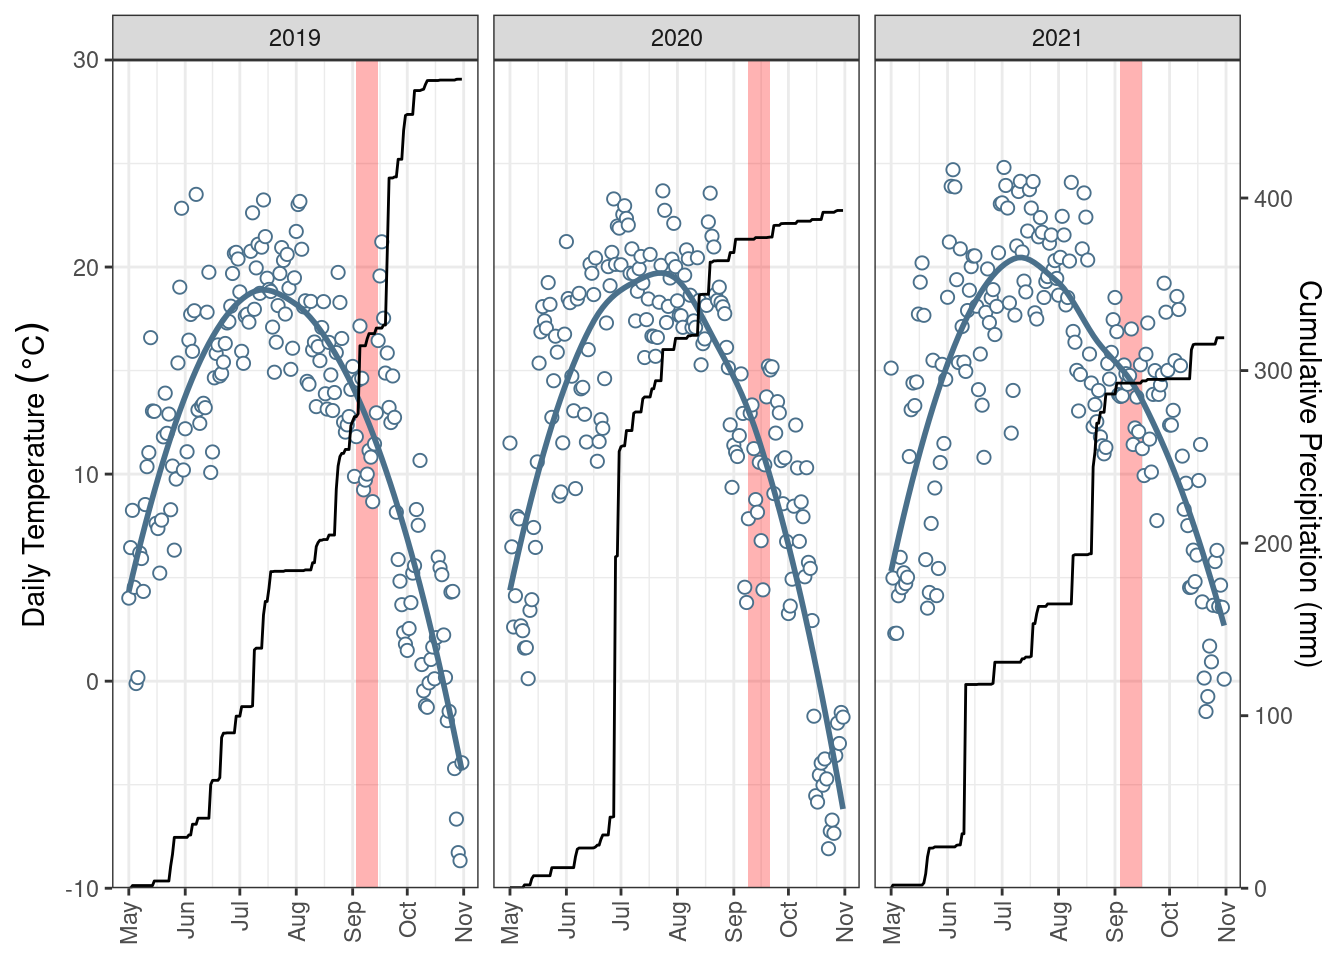
\includegraphics{supp-weather-plot-1.png}

}

\caption{\label{suppfig-weather-plot}Average daily air temperature and
cumulative rainfall over the growing season over the three year study.
Red bars indicate sampling dates}

\end{suppfig}%

\begin{suppfig}

\centering{

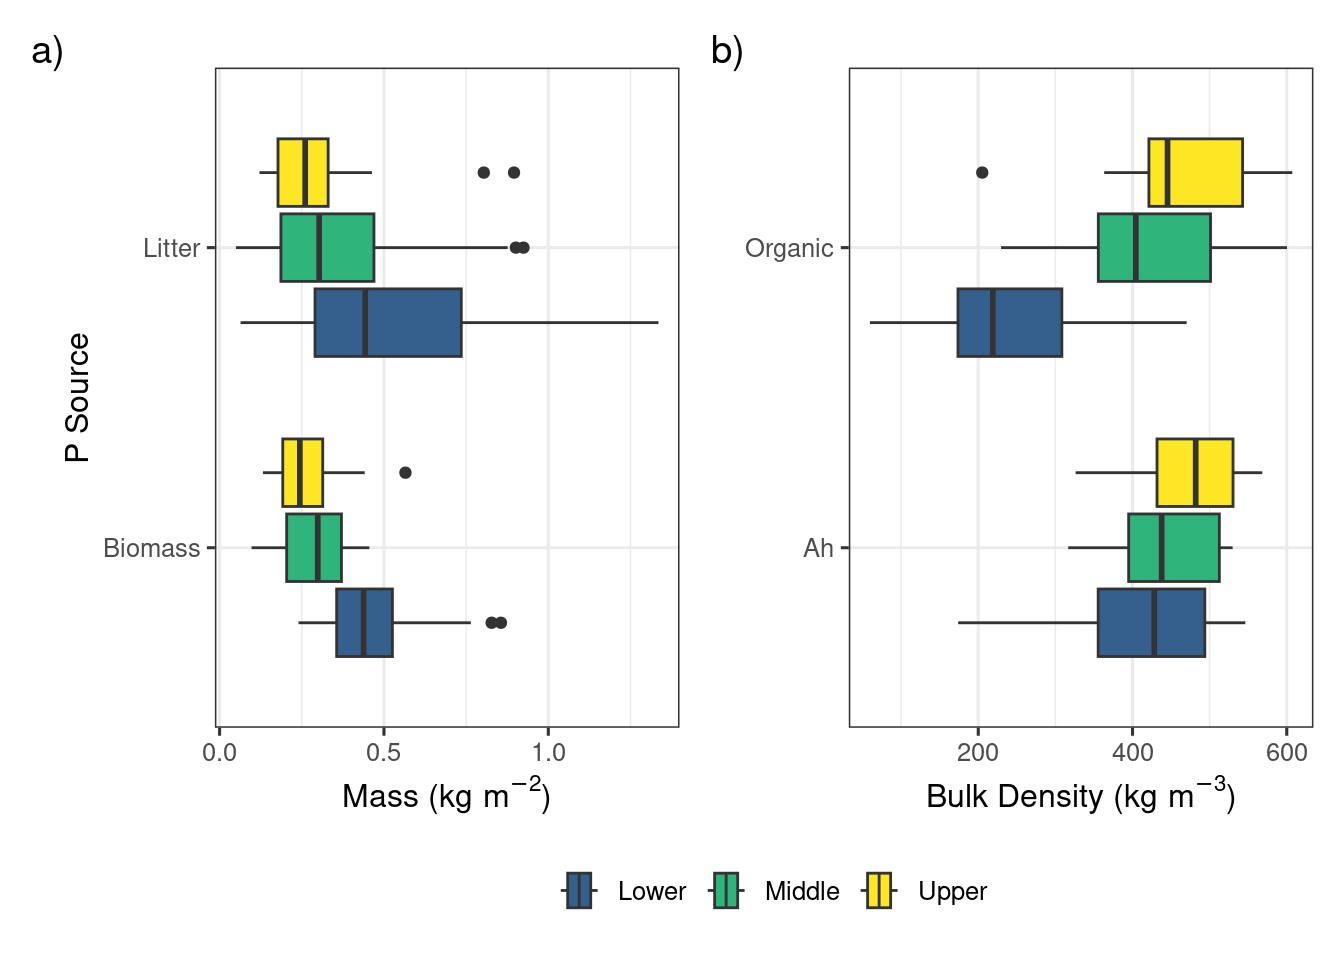
\includegraphics{supp-weights-bd-1.png}

}

\caption{\label{suppfig-bd-plot}a) Mass of biomass and litter before
grazing and mowing (2019-2021) and b) the bulk density of the organic
layer and 10 cm Ah horizon (2023)}

\end{suppfig}%



\end{document}
